\section{Experiments}
We apply SVD into two tasks, one of which is ZCA whitening and the other one is PCA denoising.
\subsection{ZCA Whitening}

The algorithm of ZCA whitening follows the big framework defined in Alg.\ref{alg: svd-foward}.
Following \cite{huang2018decorrelated}, the affine transformation operation is also kept. For simplicity, we did not show it in Alg.\ref{alg: svd-foward}.
For ZCA whitening, we have tested our algorithm on both CIFAR10 and CIFAR100 datasets.

\begin{table}[!htb]
\begin{tabular}{|l|c|c|c|c|c|c|}
\hline
Methods                 & Error & ZCA-G1                 & ZCA-G2        & ZCA-G4        & ZCA-G8        & ZCA-G16       \\ \hline
\multirow{2}{*}{SVD}    & Min   & NaN                    & NaN           & NaN           & NaN           & 4.43             \\ \cline{2-7} 
                        & Mean  & NaN                    & NaN           & NaN           & NaN           & 4.53$\pm$0.15         \\ \hline
\multirow{2}{*}{PI}     & Min   & -                      & -             & -             & -             & -             \\ \cline{2-7} 
                        & Mean  & -                      & -             & -             & -             & -             \\ \hline
\multirow{2}{*}{SVD-PI} & Min   & 4.44                   & 4.46          & \textbf{4.40} & 4.43          & 4.59          \\ \cline{2-7} 
                        & Mean  & \textbf{4.59$\pm$0.09} & 4.64$\pm$0.15 & 4.63$\pm$0.14 & 4.62$\pm$0.18 & 4.71$\pm$0.11 \\ \hline
\end{tabular}
\end{table}


\begin{table}[!htb]
\begin{centering}
\setlength\tabcolsep{2.5pt}
\begin{tabular}{|l|l|c|c|c|c|c|c|}
\hline
\multicolumn{1}{|c|}{Methods}                                                & Error & BN             & G1                  & G2                  & G4         & G8         & G16        \\ \hline
\multirow{2}{*}{\begin{tabular}[c]{@{}l@{}}CIFAR100\\ ResNet18\end{tabular}} & Min   & 21.68          & 21.04                   & 21.36                   & 21.14          & 21.15          & \textbf{21.03} \\ \cline{2-8} 
                                                                             & Mean  & 21.85$\pm$0.14 & \textbf{21.39$\pm$0.23} & 21.58$\pm$0.27          & 21.45$\pm$0.25 & 21.56$\pm$0.35 & 21.51$\pm$0.28 \\ \hline
\multirow{2}{*}{\begin{tabular}[c]{@{}l@{}}CIFAR100\\ ResNet50\end{tabular}} & Min   & 20.79          & 19.28                   & \textbf{19.24}          & 19.78          & 20.15          & 20.66          \\ \cline{2-8} 
                                                                             & Mean  & 21.62$\pm$0.65 & 19.94$\pm$0.44          & \textbf{19.54$\pm$0.23} & 19.92$\pm$0.12 & 20.59$\pm$0.58 & 20.98$\pm$0.31 \\ \hline
\end{tabular}
\end{centering}
\caption{CIFAR100 results with ResNet18 and ResNet50 as the backbone.}
\label{tab: cifar100}
\end{table}



\subsection{PCA denoising}

In the experiment, within the PCA denoising layer, we remove the noise in the feature maps by only selecting its top-$k$ eigenvectors to reconstruct the input feature maps.
We first reshape the input feature maps $X_{n {\times} c {\times} h {\times} w}$ to $X_{c {\times} nhw}$, and compute the covariance matrix $Var(X) =\frac{XX^{\top}}{nhw-1}$.
The constraint for $k$ is that $\frac{\sum_{i=1}^k\lambda_i}{\sum_{i=1}^n\lambda_i} \geq 0.95$, which means that $95\%$ of the information is preserved and the rest of the information which is lower than $5\%$ is removed. 
In practice, $k$ is relatively small compared with channel number $c$. For instance, on Cifar10 dataset, after the first convolutional layer in ResNet18 which has the channel 64, we observe that \\
more than $95\%$ of the information could be preserved when $k=7$; \\
more than $99\%$ of the information could be preserved when $k=15$; \\
more than $99.5\%$ of the information could be preserved when $k=31$. 

\subsubsection{Percentage of Preserved Information VS Performance}

\begin{figure}[!htb]
\begin{floatrow}
\ffigbox[1.1\FBwidth]{%
  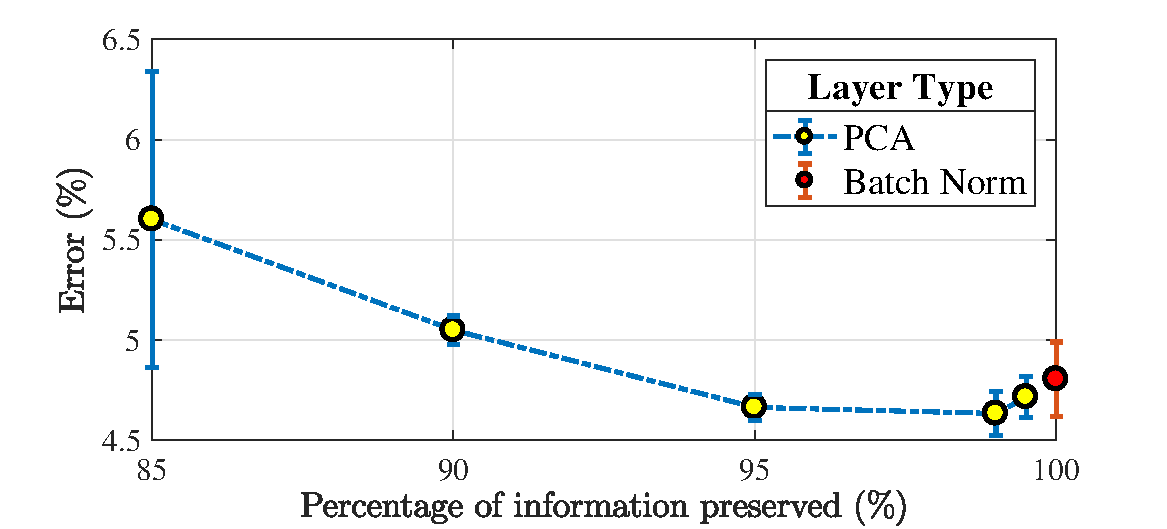
\includegraphics[width=\linewidth]{information.pdf}
}
{%
  \caption{Preserved information VS Performance.}%
}
\capbtabbox[.9\Xhsize]{%
\begin{tabular}{cc}
\hline
Percentage (\%) & Error (\%) \\ \hline
85              & $5.60\pm0.74$  \\ \hline
90              & $5.05\pm0.07$  \\ \hline
95              & $4.67\pm0.06$  \\ \hline
99              & $\mathbf{4.63\pm0.11}$  \\ \hline
99.5            & $4.72\pm0.10$  \\ \hline
100             & $4.81\pm0.19$  \\ \hline
\\
\end{tabular}
}{%
  \caption{Performance Comparison}%
}
\end{floatrow}
\end{figure}

\subsubsection{Number of EigenVectors VS Performance}

\begin{figure}[!htb]
\begin{floatrow}
\ffigbox[1.1\FBwidth]{%
  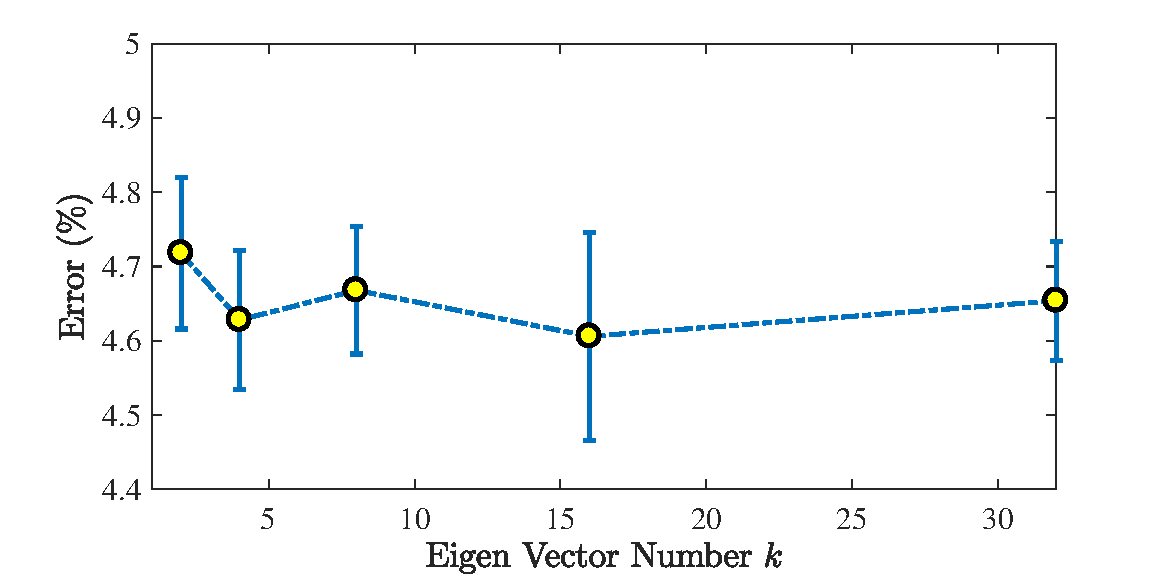
\includegraphics[width=\linewidth]{eig.pdf}
}
{%
  \caption{Eigen-vector No. VS Performance.}%
}
\capbtabbox[.9\Xhsize]{%
\begin{tabular}{cc}
\hline
Eig-vector No. & Error (\%) \\ \hline
2              & $4.72 \pm 0.10$  \\ \hline
4              & $4.63 \pm 0.09$  \\ \hline
8              & $4.67 \pm 0.09$ \\ \hline
16            & $4.61 \pm 0.14$  \\ \hline
32             & $4.65 \pm 0.08$  \\ \hline
\\
\end{tabular}
}{%
  \caption{Performance Comparison}%
}
\end{floatrow}
\end{figure}

\subsubsection{Number of Power Iterations VS Performance}

\begin{figure}[!htb]
\begin{floatrow}
\ffigbox[1.1\FBwidth]{%
  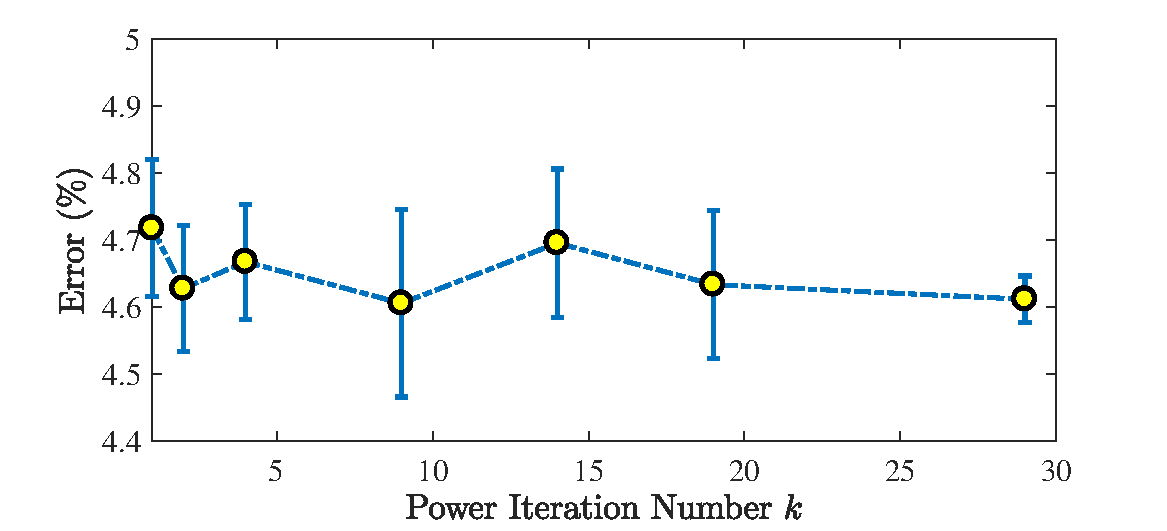
\includegraphics[width=\linewidth]{pi.pdf}
}
{%
  \caption{Power Iteration No. VS Performance.}%
}
\capbtabbox[.9\Xhsize]{%
\begin{tabular}{cc}
\hline
Power Iteration No. & Error (\%) \\ \hline
1              & $4.72 \pm 0.10$  \\ \hline
2              & $4.63 \pm 0.09$  \\ \hline
4              & $4.67 \pm 0.09$  \\ \hline
9              & $4.61 \pm 0.14$ \\ \hline
14            & $4.69 \pm 0.11$  \\ \hline
19             & $4.63 \pm 0.11$  \\ \hline
29             & $\mathbf{4.61 \pm 0.03}$  \\ \hline
\end{tabular}
}{%
  \caption{Performance Comparison}%
}
\end{floatrow}
\end{figure}

%\begin{table}[!htb]
%\begin{centering}
%\begin{tabular}{|l|c|c|c|c|}
%\hline
%Norm Methods          & BN        & PCA(PI)  & PCA(SVD) & PCA(SVD+PI) \\ \hline
%Minimum Error         & 4.66       & 5.05   & NaN   &\textbf{4.58}\\ \hline
%Mean Error (4) & $4.81{\pm}0.19$ &$5.35{\pm}0.25$ & NaN &$\mathbf{4.67{\pm}0.06}$ \\ \hline
%\end{tabular}
%\caption{CIFAR-10 test errors using ResNet18 (single PCA/ZCA normalization layer).}
%\end{centering}
%\end{table}

\begin{figure}[!htb]
\begin{floatrow}
\ffigbox[0.9\FBwidth]{%
  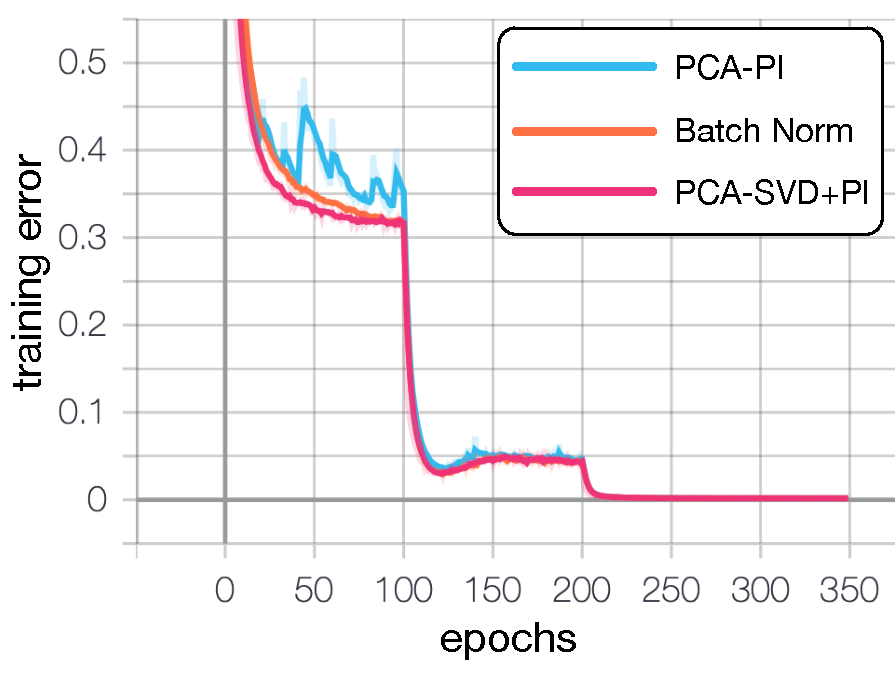
\includegraphics[width=\linewidth]{convergence.pdf}
}
{%
  \caption{Methods VS Performance.}%
}
\capbtabbox[\Xhsize]{%
\begin{tabular}{lcc}
\hline
Methods     & Min Error & Mean Error (5) \\ \hline
BN          & 4.66      & $4.81{\pm}0.19$   \\ \hline
PCA(PI)     & 5.05      & $5.35{\pm}0.25$ \\ \hline
PCA(SVD)    & NaN       & NaN                   \\ \hline
PCA(SVD+PI) & 4.58      & $\mathbf{4.67{\pm}0.06}$ \\ \hline
\\
\\
\\
\end{tabular}
}{%
  \caption{Methods VS Performance.}%
}
\end{floatrow}
\end{figure}


\begin{table}[!htb]
\begin{centering}
\begin{tabular}{|l|c|c|c|c|c|}
\hline
Norm Methods          & BN        & PCA(1 layer)   & ZCA(1 layer)  & PCA(1 block)   & ZCA(1 block) \\ \hline
Minimum Error         & 4.66      &  4.58  &   4.91 &  5.14 &  5.38\\ \hline
Mean Error (4) & $4.81{\pm}0.19$  &  $4.67{\pm}0.06$  & $5.02{\pm}0.28$ & $5.30{\pm}0.12$ & $5.50{\pm}0.10$ \\ \hline
\end{tabular}
\caption{CIFAR-10 test errors using ResNet18 (single PCA/ZCA normalization layer).}
\end{centering}
\end{table}